%# -*- coding: utf-8-unix -*-
%%==================================================
%% chapter01.tex for SJTU Master Thesis
%%==================================================

%\bibliographystyle{sjtu2}%[此处用于每章都生产参考文献]
\chapter{混合存储系统介绍}
\label{chap:hss}

\section{混合存储系统的基本概念}

混合存储系统是指利用多种不同的存储设备构建的一套数据存储系统。混合存储系统之所以存在的根本原因在于存储设备的读写性能与成本成正相关。最理想的存储系统应该是将所有的数据都存储在最高速的存储设备中,这样存储系统的性能能达到最高,但是由于同样成本下高速设备的存储容量至少要比低速设备小一个量级,因此这样的系统的成本对于一般用户而言难以接受。而混合存储系统能充分利用不同存储设备的特性,将绝大部分用户的数据存储在低速设备中,而只将用户会频繁使用的数据放在高速设备中以提供对这些数据的高存取性能,使得系统整体对外表现为大容量、高性能、高性价比。

\section{主流的存储设备的特性}

\subsection{磁盘}

磁盘,即机械磁盘,又被称为硬盘,是应用最广泛的一种存储设备。磁盘通过离磁盘片很近的磁头的电流改变磁盘片上存储的极性的方式来存储数据,数据的读取则通过与存储相反的方式进行。磁盘依照接口的不同可大致分为ATA、SATA、SCSI及SAS四种,常见的转速为每分钟4200转到每分钟10000转,工业级的高档磁盘的转速能达到每分钟15000转。磁盘的顺序读写性能与随机读写性能差异巨大,顺序读写时数据的传输速率能达到200MB/s,但随机读写时IOPS(I/O per second,即每秒的I/O操作)仅为约75,这是由于磁盘的磁头的机械移动所带来的限制,而磁盘的容量则依照摩尔定律稳步增长,因此磁盘的容量与性能的矛盾日趋严重。总的来看磁盘具有大容量、低成本、顺序读写优于随机读写的特点。

\subsection{固态盘}

固态盘(SSD:solid state disk)是使用固态电子存储芯片阵列而制成的存储设备,由控制单元和存储单元组成。SSD对存储介质的组织类似树状结构,图\ref{fig:ssd_phy}所示为三星的4GB闪存的内部组织结构\cite{agrawal2008design}。一个4GB的package由2个die(也被称为chip即芯片)组成,每个die由4个plane组成,每个plane由2048个block组成,每个block由64个4KB大小的page组成。对于不同die的操作可以并行执行,对每个die的操作最后落到1个或2个plane执行,当操作落到2个plane时,只能是plane0及plane1或plane2及plane3,而不能交叉。SSD由于不像磁盘有磁头的机械移动,而都是通过电子信号的方式,所以与磁盘相比具有体积小、质量小、能耗低、访问延迟小的特点\cite{agrawal2008design, dirik2009performance},尤其在随机读写方面比磁盘高出一个量级。虽然近年来随着工艺的进步,SSD的容量日趋提高、成本日趋下降,但与磁盘相比仍显成本高容量小,并且由于SSD有写前擦除的次数限制,耐用性方面不如磁盘,另外有研究\cite{kgil2008improving}表明如果SSD完全取代磁盘,相应的SSD垃圾回收的负载将加重,因而SSD仍无法完全取代磁盘。

\begin{figure}[!htp]
  \centering
  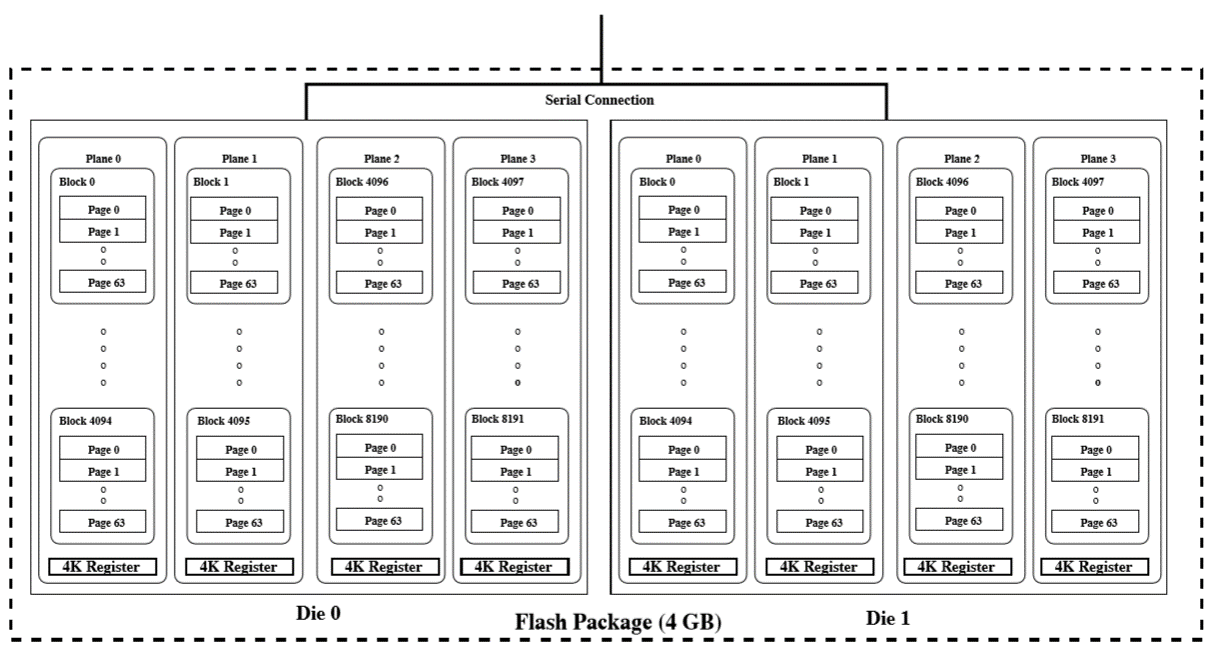
\includegraphics[width=\textwidth]{ssd_phy.png}
  \hspace{1cm}
  \bicaption[fig:ssd_phy]{固态盘存储介质的组织}{固态盘存储介质的组织}{Fig.}{organization of solid state disk storage media}
\end{figure}

\subsection{非易失性随机存储器}

非易失性随机存储器(NVRAM:Non-Volatile Random Access Memory)是指断电后仍能保持数据的一种随机访问存储器。早期的NVRAM由RAM加上电池组成,而近年来新型NVRAM已不需要电池。与SSD相比,NVRAM不存在写前擦除的操作,因此写操作比SSD更快且没有因写前擦除的次数限制带来的耐用性问题,但是与SSD相比,NVRAM的容量更小、成本更高,因此常用来作为缓存设备,而不作为主存储设备使用。

\subsection{主流的存储设备比较}

以性能、成本、容量为三大指标,磁盘、SSD、NVRAM的对比如表\ref{tab:hdd_ssd_nvram}所示。可以看到,NVRAM、SSD、HDD的性能分别为ns级、μs级(写操作为ms级)、ms级,容易分别为MB级、GB级、TB级,成本为$10^{3}$级、$10^{0}$级、$10^{-1}$级。可见不同的存储设备各有各的优势与劣势,要选取单一种类的存储设备来构建一个同时满足高性能、高容量、低成本的存储系统是极其困难的,而将不同存储设备组合起来构建混合存储设备则有可能让这些存储设备形成互补。

\begin{table}[!hpb]
    \zihao{5}
    \centering
    \bicaption[tab:hdd_ssd_nvram]{磁盘、SSD、NVRAM的对比}{磁盘、SSD、NVRAM的对比}{Table}{differences among HDD, SSD and NVRAM}
    \begin{tabular}{cccccc} \toprule
      存储设备 & 读延迟 & 写延迟 & 写前擦除延迟 & 容量量级 & \$/GB \\ \midrule
      NVRAM(FRAM) & 55ns & 55ns & N/A & $10^{0}$MB & $4 \times 10^{3}$ \\
      NVRAM(BBDRAM) & 70-100ns & 70-100ns & N/A & $10^{0}$GB & $2 \times 10^{3}$ \\
      SSD(基于闪存) & 25μs & 200μs & 1.5ms & $10^{2}$GB & $1 \times 10^{0}$ \\
      HDD(SATA接口) & 8.5ms & 9.5ms & N/A & $10^{3}$GB & $1 \times 10^{-1}$ \\ \bottomrule
    \end{tabular}
  \end{table}

\section{混合存储系统的模式}

依据混合存储系统所基于的存储设备的组合,可将混合存储系统分为不同的模式,下面对不同模式的混合存储系统分别进行介绍。

\subsection{基于NVRAM与HDD的混合存储系统}

传统上,将RAM作为HDD的缓存一直是提高存储系统整体性能的常用手段\cite{belady1966study},系统将用户频繁访问的数据放在RAM中,当访问该数据时直接从RAM中获取数据而非从HDD中获取数据,使系统对外表现为RAM的性能。然而使用RAM作为HDD的缓存只能提高系统整体的读性能,而对写性能的提升有限,这并非是由于RAM的容量相较HDD的容量太小导致缓存的容量不够用,而是由于如果发生断电,那么RAM上的数据就会丢失,而RAM作为HDD的缓存,上面可能会保有经过修改而尚未写回到HDD的脏数据,如果发生断电,那么这些数据的修改就会丢失,所以为了保证数据的可靠性,需要将RAM上的脏数据写回到HDD上,这就导致系统面临提升写性能与保障数据可靠性的两难境地。同时脏数据在RAM中驻留的时间越长,那么它再次受到改写的概率与断电带来的损失也越大,因此一般都会限制脏数据在RAM中的驻留时间,最终导致系统整体的写性能提升不显著。

NVRAM作为非易失性随机存储器,为解决将RAM作为HDD缓存的系统中脏数据的驻留时间带来的问题提供了新的解决方案。将所有的脏数据都存放在NVRAM上\cite{baker1992non},而普通数据放在NVRAM或RAM上就可以保证即使断电,数据的修改仍然能被保留,使得系统不需要频繁地将数据写回到HDD中以保证数据的可靠性,提升了系统整体的写性能。另一种作法是将NVRAM作为日志记录设备,将写操作以追加日志的形式写入NVRAM中,当NVRAM的容量使用到一定程度后再一次写回到HDD中,这样即使发生断电,系统也能从NVRAM的日志中重建出最新的数据。

总体而言,基于NVRAM与HDD的混合存储系统对于系统的可靠性问题有了比较好的解决,但对于系统整体的性能提高仍然有限。原因在于在NVRAM出现的早期阶段,NVRAM的容量小且成本高,这使得将NVRAM作为缓存,缓存容量有限,因而对系统的性能提高有限。而现在虽然NVRAM的容量在不断增长,大的NVRAM甚至能达到8GB的容量,但是与HDD的容量增长相比仍然有限,NVRAM与HDD的容量比仍在不断缩小,导致缓存的命中率不断下降,系统的性能提升的效果也在不断降低。

\subsection{基于不同转速的HDD的混合存储系统}

在20世纪90年代,产业界一度热衷于研究将不同规格不同转速的HDD组合构建混合存储系统,其基本思想也是基于将数据区分为冷热数据的想法,将用户需要经常访问的热数据放在高转速的磁盘上,而将用户不经常访问的冷数据放在低转速的磁盘上。但由于磁盘的性能瓶颈出在磁头的机械移动上,而不同转速的磁盘的磁头的机械移动并不存在显著差异,因此不同转速的磁盘构建的混合存储系统的随机读写性能并没有显著的提升。

\subsection{基于SSD与HDD的混合存储系统}

近年来,SSD的快速发展以及SSD与HDD良好的互补性,使得基于SSD与HDD的混合存储系统的研究成为存储领域的一个重要研究方向。产业界尤其表现出浓厚的兴趣,IBM\cite{ibm2010ds8000}、NetApp\cite{netapp}、EMC\cite{laliberte2009automate}等企业已经生产出了一些采用了或者支持基于SSD与HDD的混合存储的产品。

对目前已有的基于SSD与HDD的混合存储系统的研究发现SSD的写前擦除特性与擦除次数限制对系统整体的写性能影响很大,系统如果频繁地将数据写入SSD就会导致SSD的寿命减少,降低系统的可靠性,但如果频繁地将数据写入HDD则会导致系统的写性能下降,SSD无法发挥出其优势。针对这一问题,有的研究着眼于对于SSD磨损均衡的改良\cite{王增辉2015磨损均衡在提高, 李恒恒2016基于, 陈晓敏2010基于},有的研究着眼于数据冷热识别算法的研究\cite{刘庆宾2016面向多用户的, 闫林2014基于},将真正需要的数据放在SSD中。产业界中有的云存储产品就是通过使用不同转速的SSD与不同转速的HDD的组合,将原本SSD与HDD的两级架构变为更多级的架构,依据不同数据的重要程度放置在不同转速的不同存储设备上。

\subsection{基于NVRAM、SSD与HDD的混合存储系统}

上述提到基于NVRAM与HDD的混合存储系统虽然对系统的可靠性有了较好的解决但由于NVRAM与HDD的容量比问题,对系统整体性能提升有限,而基于SSD与HDD的混合存储系统由于SSD的写前擦除与擦除次数限制问题,系统的可靠性与写性能是个需要权衡的问题。因此有研究提出基于NVRAM、SSD与HDD三者的混合存储系统\cite{祝青2013混合存储系统研究},其基本思想是将NVRAM作为HDD的写缓存而将SSD作为HDD的读缓存,从而既保证了频繁的写操作不会快速消耗SSD的寿命又保证了系统的读操作命中率,由此实现了高可靠性高性能的系统,但是对于大量写操作,仍然会由于NVRAM的容量问题,使系统的写性能提升有限。

\section{混合存储系统设计中的关键技术}

目前,混合存储系统的设计中的关键技术主要有系统架构、数据映射策略、冷热数据识别算法、数据写回/迁移策略、最优化存储设备组合这五个方面,由于本文研究的主要是SSD缓存系统,因此下面针对基于SSD与HDD的混合存储系统从上述的这五个方面分别进行展开介绍。

\subsection{系统架构}

目前基于SSD与HDD的混合存储系统主要有三种系统架构:一种是分层的架构,将SSD作为HDD的缓存;另一种也是分层的架构,但是是将HDD作为SSD的缓存;最后一种是同层的架构,将SSD与HDD放在同一层,对存储系统而言,SSD与HDD是相对独立的存储设备。

\subsubsection{SSD作为HDD缓存的分层架构}

SSD作为HDD缓存的分层架构的结构如图\ref{fig:multi_layer_architecture}所示,在该架构下,SSD被完全用作HDD的缓存,混合存储系统的逻辑地址与HDD的物理地址一一对应,当混合存储系统收到来自上层的I/O请求时,首先在SSD中找寻是否存在该数据,如果存在该数据则直接在SSD中对该数据进行操作,否则会去访问HDD进行进一步操作。

在该架构下,由于SSD比RAM以及NVRAM有更大的容量,因此较RAM与NVRAM可以缓存更多数据,使得系统整体的命中率得到提升,进而提升系统整体的读写性能。然而该架构下仍然要面临SSD的寿命问题,即是将数据频繁缓存到SSD中提高性能还是将一部数据直接写到HDD中以延长SSD的寿命。

\begin{figure}[!htp]
    \centering
    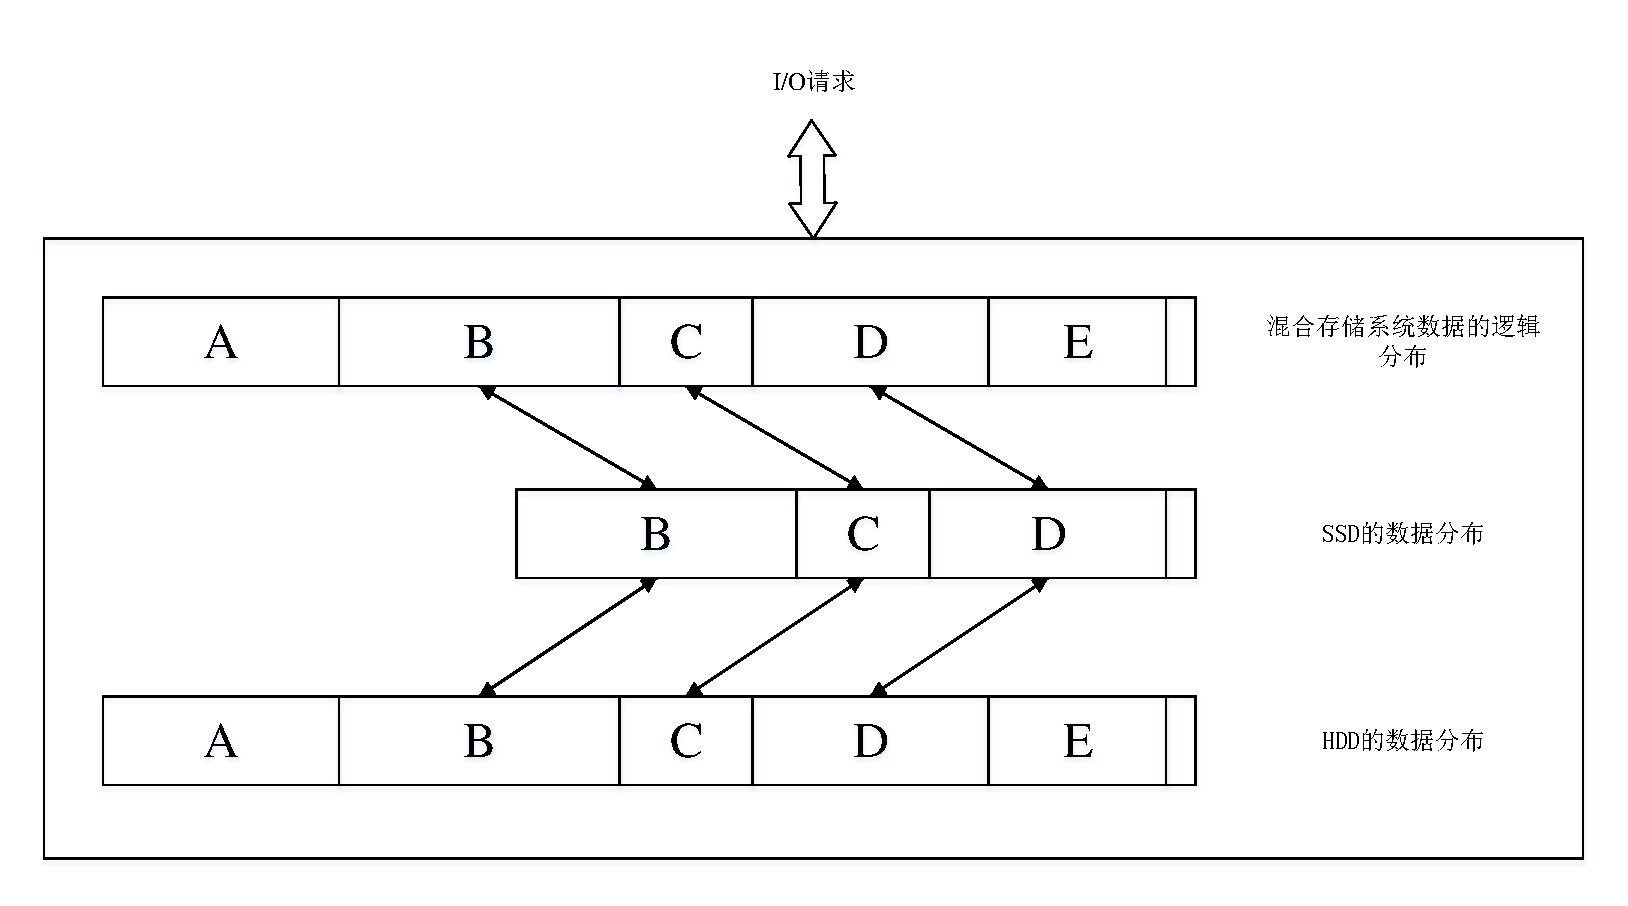
\includegraphics[width=0.8\textwidth]{multi_layer_architecture.pdf}
    \bicaption[fig:multi_layer_architecture]{分层混合存储系统架构}{分层混合存储系统架构}{Fig.}{multi-layer hybrid storage system architecture}
\end{figure}

\subsubsection{HDD作为SSD缓存的分层架构}

一般而言,SSD被用作HDD的缓存是由于其优异的随机读写性能,但是一方面存在中低端的SSD的随机读写性能反而不如一些HDD的情况,另一方面为了延长SSD的寿命,因此有的研究着眼于将HDD作为SSD的缓存\cite{soundararajan2010extending, yang2011hybrid, mao2012hpda}。在该架构下,对于SSD上数据的更新以追加日志的方式缓存在HDD上,然后根据一定的判断准则将其批量迁移回SSD。该架构主要是将大部分写操作放到HDD上进行,而让SSD处理随机读操作,以此减少对SSD的磨损并对外提供高性能。

\subsubsection{同层架构}

同层架构的结构如图\ref{fig:single_layer_architecture}所示,在该架构下,SSD与HDD处于同一层,混合存储系统的逻辑地址为SSD的物理地址与HDD的物理地址之和,当混合存储系统收到来自上层的I/O请求时会根据逻辑地址直接去找到实际存储设备的物理地址进行数据访问,但是系统会根据数据的冷热程度不同对数据进行迁移,将热数据放到SSD上而将冷数据放到HDD上。

在同层架构下,系统的整体容量为SSD与HDD的容量之和,相比分层架构提高了容量的利用率,同时根据数据冷热程度不同放到不同的存储设备上提高了系统整体的性能,但是该架构下系统的实现复杂度会较分层架构提高。

\begin{figure}[!htp]
    \centering
    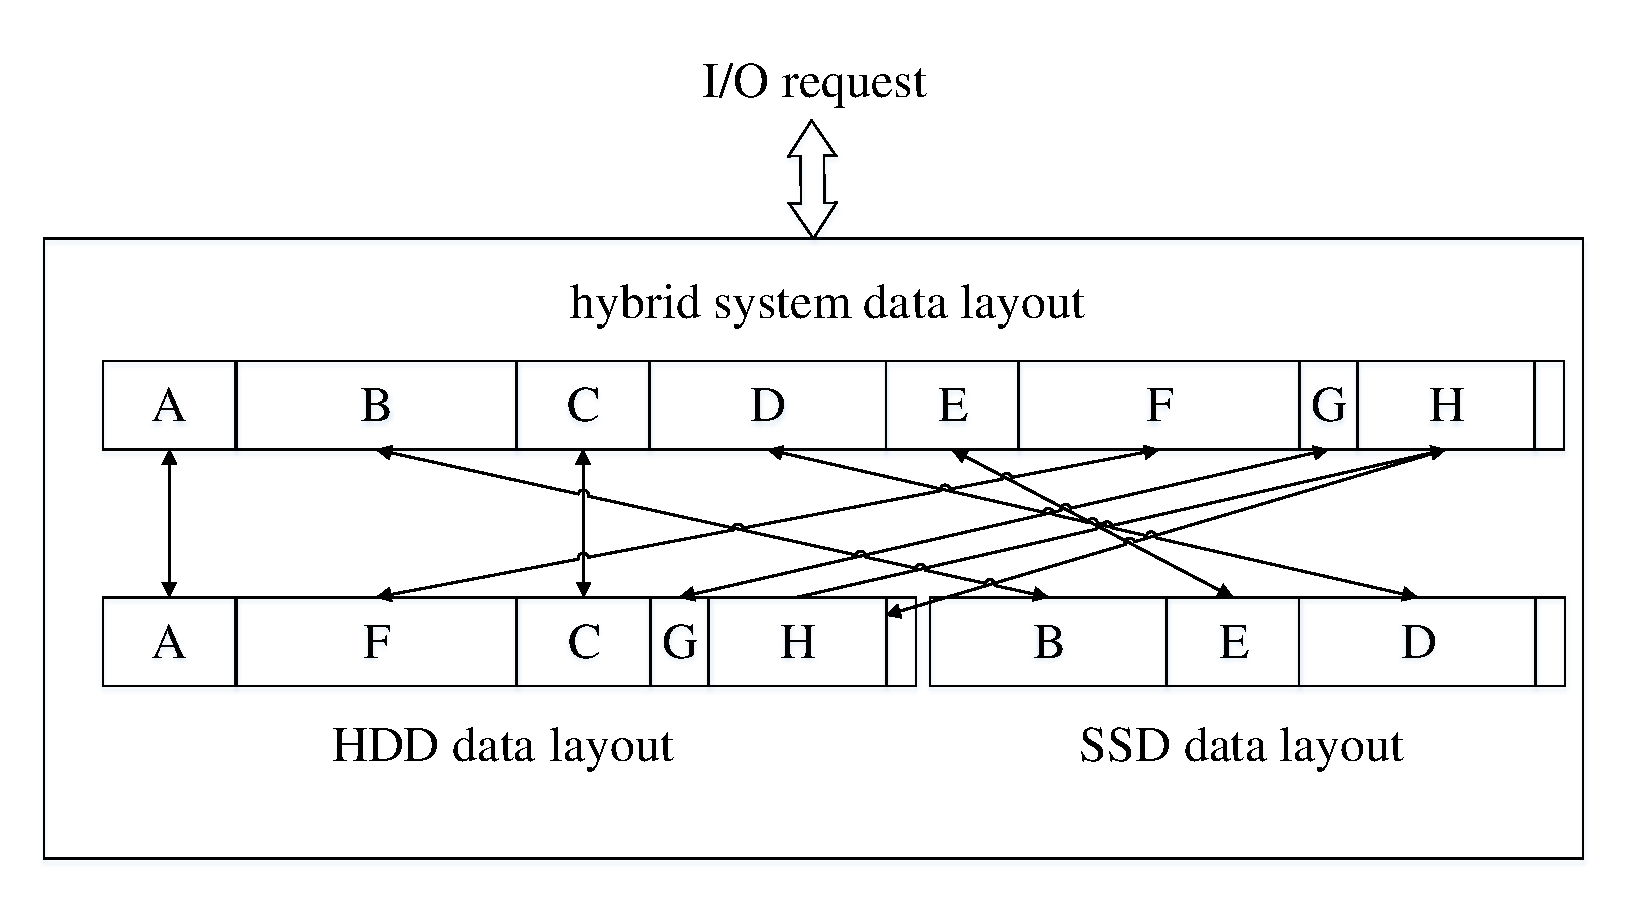
\includegraphics[width=0.8\textwidth]{single_layer_architecture.pdf}
    \bicaption[fig:single_layer_architecture]{同层混合存储系统架构}{同层混合存储系统架构}{Fig.}{single-layer hybrid storage system architecture}
\end{figure}

\subsection{数据映射策略}

无论混合存储系统是分层架构还是同层架构,最后的数据都是以块(block)为单位存放到实际设备上,因此对于每个block的I/O请求需要将其映射到具体的真实设备,这就需要考虑映射的粒度问题与映射的规则。

映射粒度是指在混合存储系统中系统能操作的数据的最小单位,它可以只是一个block的大小,也可以是多个block的大小,但应保证是block大小的整数倍。一般而言,映射粒度可分为块级、文件级与Extent级。映射规则是指混合存储系统中的逻辑地址与实际设备的物理地址的转换规则。而映射规则分为纯计算的直接映射类型、依靠映射表的全相联类型与计算和映射表混合的组相联类型三种。

\subsubsection{块级映射策略}

块级映射即以block为操作数据的最小单位。所有的实际设备以block的大小划分为多个block,对混合存储系统中的每个block的I/O请求依照特定映射规则,映射到具体的实际设备进行实际操作。一般而言,块级映射策略用于分层架构的混合存储系统中,块级映射的三种映射规则如下:全相联类型中指HDD的任一block可以映射到SSD的任一block,直接映射类型中HDD的第j块block只能通过计算映射到满足如下特定关系的SSD的第i块block中(i=j \  mod \  SSD的block数)。组相联则是首先将多个block组成一个组,HDD的组与SSD的组之间采用直接映射的方式,而组内部的块则采用全相联的方式映射。

块级映射的映射策略较为简单,且可以以最细的粒度对数据进行操作,但是粒度越细,系统的额外开销也就越大。虽然HDD映射到SSD时可以通过直接映射的方式避免映射表,但是当需要将SSD的数据写回到HDD时势必需要一张映射表才能找到正确的位置。假设SSD的容量为100GB,映射表的每个block对应的表项的大小为20bytes,那么整个映射表的大小约为500MB,并且由于映射表是频繁访问的数据,需要驻留在内存中,因此最终整个系统需要500MB的额外内存开销,这对普通用户而言已接近不可接受的额外开销大小。另外对于顺序读写请求,实际这些请求无论是全部放在SSD上进行或者都放在HDD上进行性能都相差不多,但块级映射可能会将顺序读写请求中的一些数据映射到SSD上另一些则映射到HDD上,最终导致顺序读写请求被分散到SSD和HDD上变成两个随机读写请求,这会极大影响性能。此外,在分层架构中,多个HDD的block会被映射到SSD的同一个block上,那么当发生碰撞时的处理对系统的性能影响也很大。

\subsubsection{文件级映射策略}

文件级映射即以文件为组织block的最小操作单位,同一个文件中的不同block会被映射到同一个设备上,同样,对数据的冷热识别、缓存的最小单位、数据迁移的最小单位也都是文件。相比块级映射,文件级映射的粒度显然粗很多,因此系统的额外开销会小很多,但是由于文件的大小不一,可能会存在很大的文件,当这些文件在分层架构中被缓存需要写回时或者在同层架构中需要被迁移时,系统的负载会一下子增高,而不像块级映射会比较平稳。

\subsubsection{Extent级映射策略}

Extent级映射即将多个block组成一个Extent,以Extent作为最小的操作单位,同一个Extent中的block会被映射到同一个设备上。可以认为Extent是粒度更粗的块级组相联映射,但是Extent的约束更强,Extent级映射通常是将物理连续的多个block组成一个Extent。Extent的大小可以自由指定,这就让Extent级映射变得很灵活,但同时Extent的大小十分讲究,如果设定的太小,那么系统的额外开销就会增加,同时也可能会有顺序读写性能下降的问题,而如果设定的太大,那么系统在冷热数据的识别上就会不精确,并且同样会在写回或者迁移上造成系统的负载瞬间增高。

\subsubsection{混合粒度映射策略}

混合粒度映射是指可以同时支持不同的映射粒度,目前已有研究实现了混合粒度的文件系统\cite{何耀2016面向}。混合粒度映射主要可应用于多个不同规格的缓存设备,对于不同容量的缓存设备使用不同的映射粒度,如对基于NVRAM、SSD、HDD的混合存储系统,可以设置NVRAM的粒度更细,SSD的粒度更粗,这样可以有效地减少管理映射带来的额外开销,但是相应的实现要更为复杂,尤其是对不同粒度设备上数据进行相互迁移的时候,并且如果缓存设备是单一规格,则意义不大。

\subsection{冷热数据识别算法}

冷热数据识别算法负责将数据区分为冷数据与热数据,提供将需要访问的数据放在高速设备上而将不经常访问的数据放在低速设备上的依据。冷热数据识别算法直接决定数据是否能被存在与其访问频度相符的设备上,因此冷热数据识别的准确性会直接影响系统的整体性能,冷热识别算法可大致分为块级冷热识别算法与文件/Extent级冷热识别算法,下面将分别介绍。

\subsubsection{块级冷热识别算法}

块级冷热识别算法是粒度最细的冷热识别算法,以块为冷热程度统计的最小单位。块级冷热识别算法将访问频率高的块标记为热数据,其他的标记为冷数据,由于SSD的写前擦除与擦除次数限制的特性,块级冷热识别算法在SSD的内部设计中经常有被应用以使SSD中不同块的负载均衡,使不同块的擦除次数保持平衡。

块级冷热识别算法的优势在于它真正识别出了哪些数据块是最热的数据。但是它只是给出了微观的最优解,但在宏观上未必是最优的。比如对于一组顺序读或顺序写请求,可能这组请求中涉及的数据块有的是冷数据有的是热数据,那么它们就会被存放在不同设备上,使得原本的顺序请求会被打散为在不同设备上的随机请求,这反而会降低系统的性能。

块级冷热识别的算法有很多,经典的有FIFO、LRU等算法,这些算法虽然计算简单、实现简单,但是热点识别的准确率不高,比如当发生一个很长的循环遍历时,FIFO或者LRU的队列或者链表会被反复替换,导致系统的性能下降。近年来出现了不少不仅仅依赖于访问时间的冷热识别算法,如ARC\cite{megiddo2003arc}、Clock-Pro\cite{jiang2005clock}、多哈希函数\cite{hsieh2006efficient}、多布隆过滤器\cite{park2011hot}、WDAC\cite{park2011hot}等算法。这些新算法通过使用新近性和频度来判断数据的冷热程度,虽然增加了额外的开销和提高了实现的复杂度,但是提高了热点识别的准确率,并且能够抵抗循环遍历造成的热点冲刷。另外,随着SSD的兴起,近年来出现了许多针对SSD磨损均衡的冷热识别算法的研究,如CCF-LRU\cite{li2009ccf}、PUD-LRU\cite{hu2010pud}等。

\subsubsection{文件/Extent级冷热识别算法}

文件/Extent级冷热识别算法以文件或者Extent为冷热程度统计的最小单位。每个块的I/O请求都会影响该块所属的文件或Extent的热度,同时除了文件或Extent中块的访问频率,该粒度下还可引入文件或Extent中热点块的分布、带宽等更宏观的指标来对更新文件或Extent的冷热程度。

文件/Extent级冷热识别算法的优势在于与块级冷热识别算法相比,更粗的粒度能带来更小的系统额外开销,并且可以同时从微观与宏观两个方面进行热点识别,能够识别出顺序读写请求与随机读写请求,以此为依据避免将顺序读写请求打散到不同设备上。但是文件/Extent级的冷热识别算法下一般会对应地以文件或Extent为最小操作单位,由此可能会引发在数据映射中提到的问题。

\subsection{数据写回/迁移策略}

在混合存储系统中最理想的情况是将热数据都存放在高速设备上,而将冷数据放在低速设备上,但由于数据的冷热程度会不断变化,并且高速设备的容量有限可能并不能存放所有热数据,因此会发生数据不处在与其冷热程度匹配的设备的情况,数据写回/迁移策略就是负责将数据迁移到与其冷热程度匹配的设备上,以提高系统整体的性能。数据写回/迁移策略需要考虑哪些数据需要写回/迁移、何时写回/迁移这些数据这两个个问题。

写回/迁移数据的选择根据冷热识别算法决定,一旦冷热识别算法确定,通过该算法就能直接确定哪些热数据处在低速设备上,哪些冷数据处在高速设备上,针对这些数据再以对应的粒度:块级、文件级、Extent级生成待写回/迁移的数据集合即可。

数据的写回/迁移时机大致可分为静态与动态两种策略。静态策略是指系统周期性地对数据进行写回或迁移,静态策略一般选择在系统负载轻的时候(如半夜之后)进行大规模的写回/迁移,因此系统的性能波动对外影响较小,但是静态策略无法及时针对数据的冷热变化作出响应,无法实时达到系统的理论最大性能。动态策略是指不定期地对数据进行写回或迁移以对数据的冷热变化作出实时响应,动态策略可以保证系统的性能一直保持尽可能高,但是动态策略可能会让系统的性能波动变大,并且在系统重负载时影响到对外性能,尤其是当粒度为文件/Extent级时,甚至可能导致系统对外表现为不可用的状态。

\subsection{最优化存储设备组合}

最优化存储设备组合是指在保证系统达到性能需求的前提下尽可能降低系统的成本,这也是混合存储系统设计中要考虑的问题。该问题需要考虑系统架构、系统负载类型、存储设备的特性等诸多因素。该问题的解决可分为静态策略与动态策略两种。

\subsubsection{静态策略}

静态策略是指在构建混合存储系统的时候就选取好不同存储设备的型号、数量等,在混合存储系统上线运行后就不再变更,如果需要变更,则需要先将系统停止后更改配置再运行。目前静态策略的生成分为通过模拟\cite{guerra2011cost}给出最优解与通过理论推导计算\cite{kim2011hybridstore}给出最优解两种。静态策略的优势在于实现简单,配置与混合存储系统相对独立,但缺点在于不能实时适应对系统的需求。

\subsubsection{动态策略}

动态策略是指在混合存储系统运行过程中能够不需要停止运行就能重新适应用户的新需求,比如在系统运行的过程中对存储设备的热插拔,在系统运行过程中冷热数据识别算法或者数据写回/迁移策略的动态变更等等。动态策略的优势在于可以实时适应系统上负载的变化以达到最高的性能,但缺点在于要实现动态策略比较复杂,尤其是动态的设备添加或删除,需要在混合存储系统的实现中对设备的管理、数据映射做出比较大的改变。

\section{本章小结}

本章首先介绍了混合存储系统的基本概念,然后介绍了目前主流的存储设备的特性,并对比分析了这些主流存储设备在性能、容量、成本方面的差异。最后对几种不同的混合存储系统的模式做了简单的介绍,对发展中不同混合存储系统的优劣进行了简单的阐述。对于这些混合存储系统的优劣将引出了混合存储系统中的关键技术。对于混合存储系统设计中的关键技术首先介绍了系统架构,对分层架构和同层架构进行了阐述;然后介绍了数据映射策略,对块级、文件级、Extent级三种不同映射策略进行了介绍与对比分析;之后介绍了冷热数据识别算法;然后对数据写回/迁移策略从静态与动态两种策略进行了对比分析;最后介绍了最优化存储设备组合。